\documentclass[11pt]{article}

% --- Packages ---
\usepackage[a4paper,margin=1in]{geometry}
\usepackage{amsmath,amssymb,amsthm}
\usepackage{lmodern}
\usepackage{microtype}
\usepackage{bbold}
\usepackage{placeins}
\usepackage{graphicx}

% --- Title info ---
\title{MATH-517: Assignment 3}
\author{Giorgio Panizzutti}
\date{}

\begin{document}
\maketitle


\section*{1. Theoretical Exercise}
\subsection*{1.1.}
The problem is a weighted least squares problem at x:
\[
(\hat\beta_0(x),\hat\beta_1(x))
=\arg\min_{\beta_0,\beta_1\in\mathbb{R}}
\sum_{i=1}^n \left(Y_i-\beta_0-\beta_1(X_i-x)\right)^2
K\left(\frac{X_i-x}{h}\right).
\]
with
\[
X=\begin{pmatrix}
1 & X_1-x\\
\vdots & \vdots\\
1 & X_n-x
\end{pmatrix},\quad
W=\mathrm{diag}(K\left(\frac{X_1-x}{h}\right),\ldots,K\left(\frac{X_n-x}{h}\right)),\quad
Y=\begin{pmatrix}Y_1\\ \vdots\\ Y_n\end{pmatrix}.
\]
The problem can be rewritten as
\[
(\hat\beta_0(x),\hat\beta_1(x))
=\arg\min_{\beta_0,\beta_1\in\mathbb{R}}
(Y-X\beta)^{\top}W(Y-X\beta),
\]
The weighted least squares solution is
\[
\begin{pmatrix}\hat\beta_0(x)\\ \hat\beta_1(x)\end{pmatrix}
=(X^{\top}WX)^{-1}X^{\top}WY.
\]
Let \(e_1=(1,0)^{\top}\). Then
\[
\hat m(x)=\hat\beta_0(x)=e_1^{\top}(X^{\top}WX)^{-1}X^{\top}WY
=\sum_{i=1}^n w_{ni}(x)\,Y_i,
\]
where \(w_{ni}(x)\) is the \(i\)-th entry of the row vector \(e_1^{\top}(X^{\top}WX)^{-1}X^{\top}W\).
\subsection*{1.2.}
Using the notation
\[S_{n,k}(x) = \frac{1}{nh} \sum_{i=1}^n (X_i - x)^k K\left(\frac{X_i-x}{h}\right)\]
we can write 
\[X^{\top}WX = nh \begin{pmatrix}
S_{n,0}(x) & S_{n,1}(x)\\
S_{n,1}(x) & S_{n,2}(x)
\end{pmatrix}.\]
The inverse is
\[(X^{\top}WX)^{-1} = \frac{1}{nh(S_{n,0}(x)S_{n,2}(x)-S_{n,1}(x)^2)}
\begin{pmatrix}
S_{n,2}(x) & -S_{n,1}(x)\\
-S_{n,1}(x) & S_{n,0}(x)
\end{pmatrix}.\]
then 
\(X^{\top}W\) is the \(2\times n\) matrix
\[
X^{\top}W=
\begin{pmatrix}
K\left(\frac{X_1-x}{h}\right) & \cdots & K\left(\frac{X_n-x}{h}\right)\\
(X_1-x)K\left(\frac{X_1-x}{h}\right) & \cdots & (X_n-x)K\left(\frac{X_n-x}{h}\right)
\end{pmatrix}.
\]
the product \((X^{\top}WX)^{-1}X^{\top}W\) is then
\[
\frac{1}{nh(S_{n,0}(x)S_{n,2}(x)-S_{n,1}(x)^2)}
\begin{pmatrix}
(S_{n,2}(x) - (X_1 - x) S_{n,1}(x))K\left(\frac{X_1-x}{h}\right) & \cdots & \\
(-S_{n,1}(x) + (X_1 - x) S_{n,0}(x))K\left(\frac{X_1-x}{h}\right) & \cdots &
\end{pmatrix}
\]
The \(i\)-th entry of the first row is then

\[
w_{ni}(x) = \frac{1}{nh}\frac{S_{n,2}(x) - (X_i - x) S_{n,1}(x)}{S_{n,0}(x)S_{n,2}(x)-S_{n,1}(x)^2} K\left(\frac{X_i-x}{h}\right).
\]

\subsection*{1.3.}
The sum of the weights is
\[
\sum_{i=1}^n w_{ni}(x)
=\frac{1}{nh}\,
\frac{S_{n,2}(x)\sum_{i=1}^n K\left(\frac{X_i-x}{h}\right)
- S_{n,1}(x)\sum_{i=1}^n (X_i-x)K\left(\frac{X_i-x}{h}\right)}
{S_{n,0}(x)S_{n,2}(x)-S_{n,1}(x)^2}.
\]
Since \(\sum_{i=1}^n K\left(\frac{X_i-x}{h}\right)=nh\,S_{n,0}(x)\) and
\(\sum_{i=1}^n (X_i-x)K\left(\frac{X_i-x}{h}\right)=nh\,S_{n,1}(x)\),
We have 
\[\sum_{i=1}^n w_{ni}(x) =
\frac{S_{n,2}(x)S_{n,0}(x)-S_{n,1}(x)^2}
{S_{n,0}(x)S_{n,2}(x)-S_{n,1}(x)^2}=1.\]    

\section*{2. Practical Exercise}

The goal is to understand how the global bandwidth \(h_{AMISE}\)
\[
h_{AMISE}=n^{-1/5}\left(\frac{35\sigma^2|\mathrm{supp}(X)|}{\theta_{22}}\right)^{1/5},
\qquad 
\theta_{22}=\int \{m''(x)\}^2 f_X(x)dx,
\]
behaves when we change specific quantities in the estimation:
(i) the number of blocks \(N\) used to estimate \(\sigma^2\) and \(\theta_{22}\) with blockwise quartic OLS,
(ii) the sample size \(n\),
and (iii) the shape of the covariate distribution \(X\sim\mathrm{Beta}(\alpha,\beta)\).
We keep \(\sigma^2=1\) and \(|\mathrm{supp}(X)|=1\) since \(X\in[0,1]\).
The regression curve is \(m(x)=\sin((x/3+0.1)^{-1})\).


We generate i.i.d. samples \(\{(X_i,Y_i)\}_{i=1}^n\) with \(Y_i=m(X_i)+\varepsilon_i\), \(\varepsilon_i\sim\mathcal N(0,\sigma^2)\).
To estimate the unknown \(\theta_{22}\) and \(\sigma^2\) we split the sample into \(N\) blocks by quantiles of \(X\) so that each block has (almost) the same number of observations even when \(X\) is skewed. In each block \(j\) we fit
\[
y=\beta_{0j}+\beta_{1j}x+\beta_{2j}x^2+\beta_{3j}x^3+\beta_{4j}x^4+\epsilon,
\]
and then compute
\[
\hat{\theta}_{22}(N)=\frac{1}{n}\sum_{i=1}^n\sum_{j=1}^N \{\hat m_j''(X_i)\}^2 \mathbb{1}_{\{X_i\in X_j\}},\qquad
\hat\sigma^2(N)=\frac{1}{n-5N}\sum_{i=1}^n\sum_{j=1}^N \{Y_i-\hat m_j(X_i)\}^2 \mathbb{1}_{\{X_i\in X_j\}}.
\]
We plug \(\hat\sigma^2(N)\) and \(\hat\theta_{22}(N)\) in the formula for \(h_{AMISE}\).
When we need to choose \(N\) from data we use Mallow's \(C_p\)
\[
C_p(N)=\frac{\mathrm{RSS}(N)}{\mathrm{RSS}(N_{\max})/(n-5N_{\max})}-(n-10N),
\quad N_{\max}=\max\{\min(\lfloor n/20\rfloor,5),1\},
\]
and pick the minimizer over \(N=1,\dots,N_{\max}\).

We average over \(R=200\) repetitions to get stable estimates of \(\hat h_{AMISE}\).


\paragraph{Effect of the block count.}
Figure~\ref{fig:q1} shows, for \(n=2000\), the mean and standard deviation of \(\hat h_{AMISE}\) as \(N\) increases for three shapes of \(X\): \(\mathrm{Beta}(2,2)\) (symmetric), \(\mathrm{Beta}(1,4)\) (mass near \(0\)), \(\mathrm{Beta}(4,1)\) (mass near \(1\)).
In all cases \(\hat h_{AMISE}\) decreases with \(N\).
This is expected: larger \(N\) makes each of the quartic polynomial fits concern a smaller region, which increases \(\hat{\theta}_{22}\) (sum of squared second derivatives evaluated across the sample).
Since \(\hat h_{AMISE}\propto(\hat\sigma^2/\hat\theta_{22})^{1/5}\) and \(\hat\sigma^2\) is fairly stable, \(h_{AMISE}\) goes down.

\begin{figure}[h]
\centering
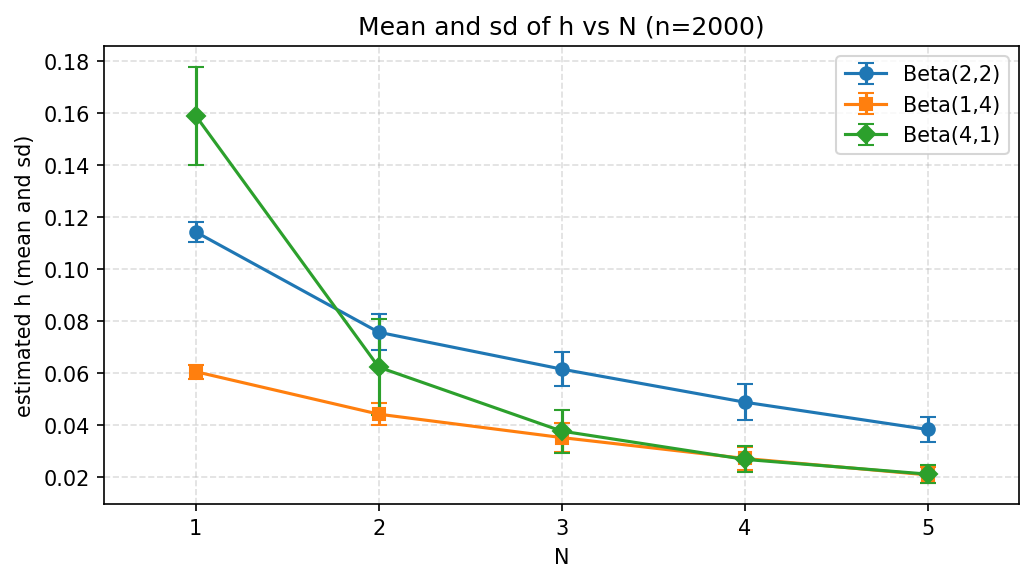
\includegraphics[width=.85\linewidth]{output/h_vs_N_mean.png}
\caption{Mean with standard deviation of \(\hat h_{AMISE}\) versus \(N\) for \(n=2000\) using three Beta distributions.}
\label{fig:q1}
\end{figure}
\FloatBarrier

\paragraph{Does optimal \(N\) depend on \(n\)?}
Figure~\ref{fig:q2} reports the average \(N\) selected by \(C_p\) as a function of \(n\) for the same three Beta shapes, with bands showing the standard deviation across replications.
There is a clear increasing trend: as \(n\) grows, the selected \(N\) increases slowly.
In the symmetric case \(\mathrm{Beta}(2,2)\), the average selected \(N\) grows roughly logarithmically with \(n\), so the trend appears linear on a log scale.
For the skewed cases (\(\mathrm{Beta}(1,4)\) and \(\mathrm{Beta}(4,1)\)), the selected \(N\) grows less.
There is a large difference between the two skewed cases: when the mass of \(X\) is near \(0\) (\(\mathrm{Beta}(1,4)\)) the selected \(N\) is much larger than when mass is near \(1\) (\(\mathrm{Beta}(4,1)\)).
This is because \(m\) has higher curvature near \(0\), and more blocks may help to capture it better, with a larger \(n\) we get a larger number of samples across the whole support, covering better the less sampled regions.
Also, having more values for each block helps to estimate the local function shape better, so greater \(n\) allows for larger optimal \(N\).

\begin{figure}[h]
\centering
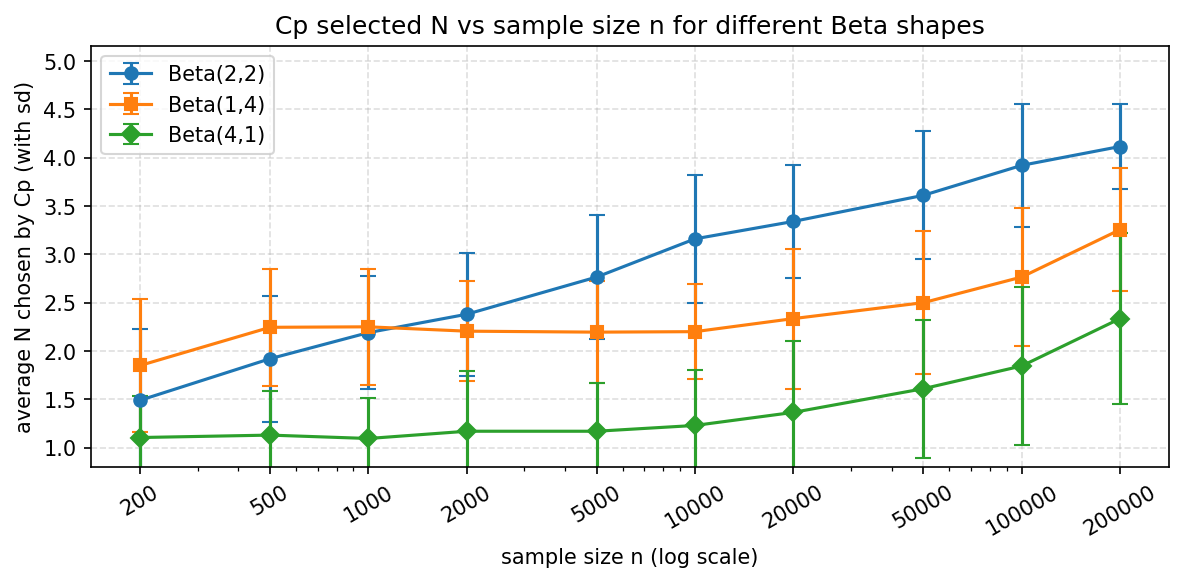
\includegraphics[width=.95\linewidth]{output/avgN_vs_n.png}
\caption{Average \(N\) selected by \(C_p\) versus \(n\) for \(\mathrm{Beta}(2,2)\), \(\mathrm{Beta}(1,4)\), and \(\mathrm{Beta}(4,1)\); bands show the standard deviation across \(R=200\) repetitions.}
\label{fig:q2}
\end{figure}
\FloatBarrier

\paragraph{Impact of the covariate Beta distribution.}
Figure~\ref{fig:q3} shows a heatmap of the mean \(\hat h_{AMISE}\) over a grid of different values of \(\alpha\) and \(\beta\) for \(n=1000\).
The largest \(h_{\mathrm{AMISE}}\) occur for large \(\alpha\) and small \(\beta\) (mass near \(1\)), while the smallest occur for small \(\alpha\) and large \(\beta\) (mass near \(0\)).
This matches the geometry of \(m\), curvature is highest near zero.
When the density of \(X\) has more probability where \(|m''(x)|\) is large, \(\theta_{22}=\int m''(x)^2 f_X(x)\,dx\) increases and the optimal \(h\) decreases. 
When more mass is in flatter regions, \(\theta_{22}\) is smaller and \(h_{AMISE}\) increases.

\begin{figure}[h]
\centering
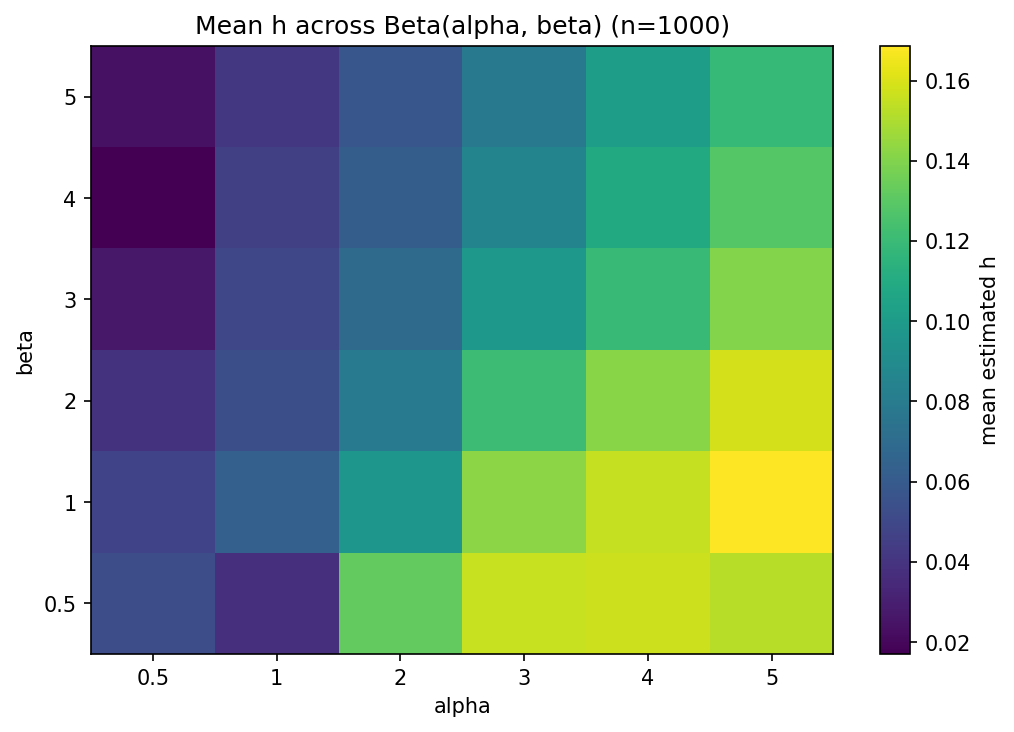
\includegraphics[width=.9\linewidth]{output/heatmap_h_by_alpha_beta.png}
\caption{Mean \(\hat h_{AMISE}\) on a grid of \(\mathrm{Beta}(\alpha,\beta)\) distributions for \(n=1000\).}
\label{fig:q3}
\end{figure}
\FloatBarrier


\paragraph{Second derivative of \(m\).}
To better see why \(h_{AMISE}\) varies with the distribution of \(X\), we plot \(m(x)\) and its second derivative \(m''(x)\) on \([0,1]\).
The curvature is highest near \(x=0\) and decreases toward \(x=1\), so \(\theta_{22}=\int m''(x)^2 f_X(x)dx\) increases when more probability mass is placed near \(0\).

\begin{figure}[h]
\centering
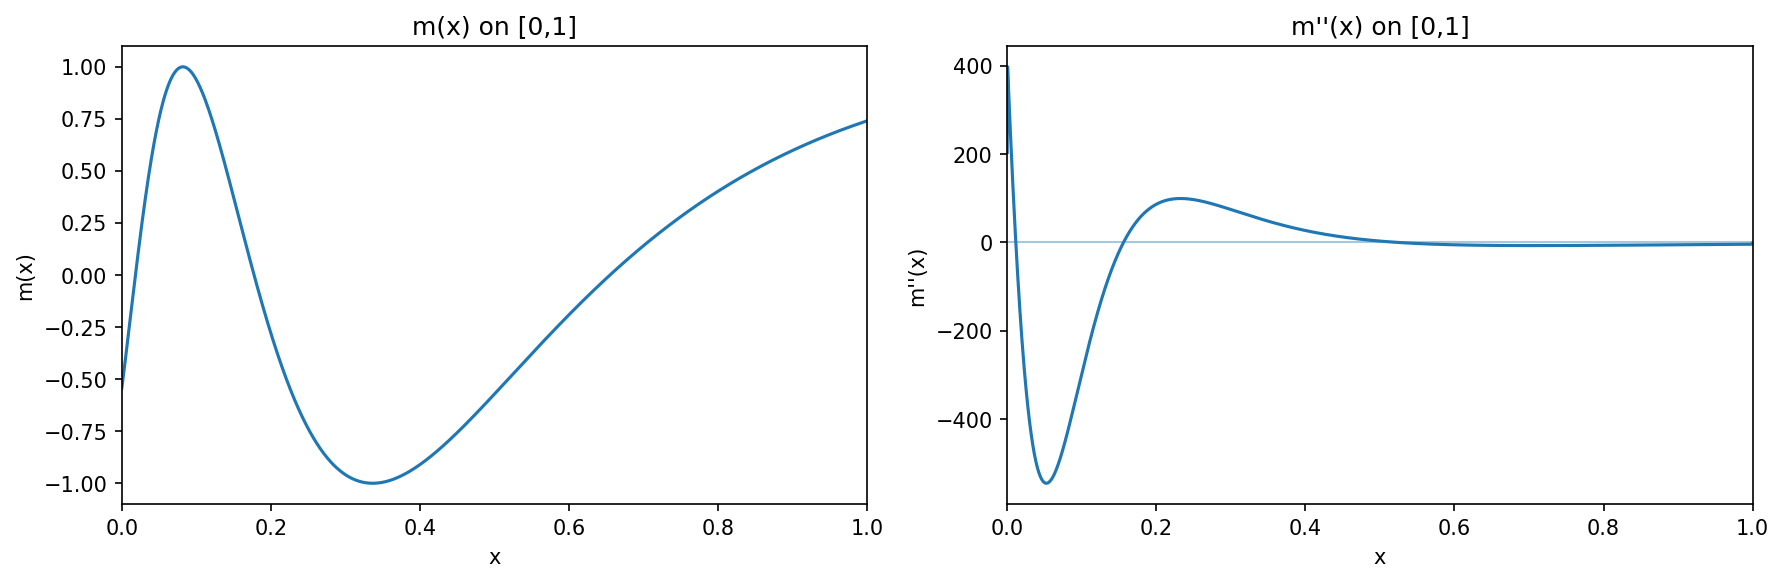
\includegraphics[width=.9\linewidth]{output/m_and_mpp.png}
\caption{Regression function \(m(x)\) (left) and its second derivative \(m''(x)\) (right) on \([0,1]\).}
\label{fig:m_mpp}
\end{figure}
\FloatBarrier



\end{document}